\chapter{结构}
\label{chp:structure}

\begin{quotation}
善张网者引其纲,不一一摄万目而后得。
\begin{flushright}
--- 《韩非子·外储说右下》
\end{flushright}
\end{quotation}

在 \ref{sec:structure} 节中我们曾简略提及文档的结构,本章将对它们展开介绍。通常一篇文档无论长短都会有标题和正文。如果正文较长,有个层次结构会便于行文,阅读起来也较方便。为了便于查找,长文档通常会前有目录,后有索引。另外为了便于编辑,长文档通常会被分割成多个文件。和 HTML 类似,PDF 也提供超链接功能,它也放在本章介绍。学术文档一般还会有参考文献,以供读者参考、借鉴。

以上诸项通常会按标题、目录、正文、参考文献、索引这样的顺序出现。如果是正式出版的书籍,还会有标题页、版权页、献辞页等;而且这些结构出现的奇偶页也有讲究,比如版权页是偶数页,目录首页是奇数页。同学们若对书籍的格式装帧有兴趣,可以参考 Peter R. Wilson\indexWilson{} \footnote{剑桥大学机械学士,诺丁汉大学半导体物理博士。本科毕业后就职于不列颠托马森休斯顿公司 (British Thomson Houston) ;后跳槽到卢卡斯研究中心 (Lucas Research Center) 搞CAD,曾任计算机辅助制造国际 (Computer-Aided Manufacturing International, CAM-I) 欧洲分部主席;再跳槽到GE参与开发CAD/CAM数据交换标准STEP;又跳槽到RPI、美国天主教大学 (Catholic University of America) 、国家标准技术研究所 (National Institute of Standards and Technology, NIST) 等院所从事科研,最后从波音退休。} 的\emph{Notes on Book Design}\citep{Wilson_2009}和\emph{Memoir Class}\citep{Wilson_2010},或者\emph{Chicago Manual of Style}\citep{Chicago_2003}。

\section{长文档}

文章想要吸引读者就必须写得好,想要影响深远就必须写得长。包子曰:神奇卓异非至人,至人只是长。当文档很长时,我们最好把它分为多个文件,各个击破,从而缓解长期伏案写作带来的悲观厌世情绪。这和高速公路上为了防止疲劳驾驶设置的技术弯道有异曲同工之妙。

\autoref{exa:include} 示范了如何在主控文档中引用子文档。注意 \verb|\include| 命令会新起一页,如果不想要新页可以改用 \verb|\input| 命令。

\begin{example}[h]
\begin{Code}[]
%master.tex
\begin{document}
\chapter{LaTeX入门}
\begin{lstlisting}[language={[LaTeX]TeX}]
	\documentclass={article}
	\begin{document}
	\end{document}
\end{lstlisting}
	\section{了解LaTeX并及其相比传统字处理软件的优缺点}
	\section{安装一个包括编辑器在内的完整的LaTeX套件}
	\section{写第一份LaTeX文档}

\chapter{字,行,段的格式化}
在上一章中,我们安装了LaTeX和TEXworks的编辑器来编写我们的
第一个文档。现在,我们将谈论的文档结构,我们
将重点放在文本的细节和它的格式。

在这一章中,我们将:
\begin{itemize}
	\item 探讨关于逻辑格式化
	\item 学习如何更改字体,文本的形状和风格
	\item 使用box来限制文档的宽度
	\item 学习如何断行和提高断字
	\item 探索对齐和格式化段落
\end{itemize}

过工作的例子,并尝试新的功能,我们将学习一些基本概念
乳胶。通过本章的结束,我们将命令和环境的熟悉。
你甚至可以定义自己的命令。
	\section{理解逻辑格式化}
在前面的章节中,我们写了一个小例子文件。让我们扩展它使得它变成一个具有
说明性的例子,以了解典型的文档结构。
		\subsection{Time for action-titling your document}
我们将使用第一个例子,插入一些命令使其产生一个漂亮的title。
\begin{lstlisting}[language={[LaTeX]TeX}]
\documentclass[a4paper,11pt]{article}
\begin{document}
\title{Example 2}
\author{My name}
\date{January 5, 2011}
\maketitle
\section{What's this?}
This is our second document. It contains a title and a section
with text.
\end{document}
\end{lstlisting}
\begin{itemize}
	\item 我们的文档使用article类。它将使用a4纸和11号基本字体。
	\item 标题是"Example 2".
	\item 你是作者。
	\item 时间是January 5, 2011
	\item concerning the content of the document:
		\begin{itemize}
			\item 开始与标题。
			\item 第一section具有标题"What's this?"
			\item 接下来的文本是"This is our second document."
		\end{itemize}
\end{itemize}
注意,我们并没有设置标题的字体大小;页眉有设置加粗和居中。这类的格式化是LaTeX
做的,但是你可以告诉LaTeX具体看起来效果如何。
		\subsection{探索文档结构}
让我们看看细节。一个LaTeX文档中并不是孤立的-通常是基于一个
多功能的模板。这类基本的模板被称为类(class)。它提供了可定制的
功能,通常是具有特定的目的性。有些类中有书(book),期刊文章
(journal articles);信件(letter),演示文档(presentation),海报
(poster)和其他很多;还有更多的数百个可靠的类可以在互联网存档,
在你已经安装了TeX Live之后,在您的计算机上也有很多,在这里,我们
选择了适用于小型文档的文章(article)类别。

第一行用\textbackslash documentclass开始。这个单词之前有反斜杠;这样的单词称为
命令(command)。我们使用命令制定类(class)和文档属性(document properties):
title,author和date.

文档的第一布冯称为文档的前言(preamble)。我们在这里选择类,指定属性,
一般地,在这里制作整个文档范围的定义。

\textbackslash begin\{document\}标记了前言的结束和真正文档的开始.\textbackslash end\{document\}标记了文档的结束。所有之后的东西都将被LaTeX忽略。在\textbackslash begin...\textbackslash end之间的这样一段代码,被称作环境(environment)。

在实际的文档中间,我们使用了\textbackslash maketitle来以一种美观的格式输出标题,作者和日期。
使用\textbackslash section命令,我们制作了一个比正常文字大且粗的标题。接着是一些文字,
在文档环境中的将被输出。相反的,前言从来不产生任何输出。

让我们仔细看一下这些命令。

		\subsection{理解LaTeX命令}
LaTeX命令以反斜杠开始,跟着是一串大写或小写字母。LaTeX命令通常使用一种
描述性的小写字符串命名。当然也有例外:你将会看到有些命令只有反斜杠和一个特殊
字符组成。

命令也可以有参数,含在大括号或方括号中。

调用命令格式如下:

\textbackslash command

或者:

\textbackslash command\{argument\}

或者:

\textbackslash command\[optionan argument\]\{argument\}

参数可以有多个,每个在大括号或方括号内。在大括号中的参数是必需的。如果一个
命令被定义为需要一个参数,那么就必须提供一个。例如,如果我们没有声明一个类名,
调用\textbackslash documentclass将是徒劳的,

%这些内容是大括号中的
方括号中的参数是可选的,如果不指定的话,会使用默认设置,例如\textbackslash documentclass\{article\}.
这份文档将使用10pt字体,因为这是这个类的默认值。
\textbackslash documentclass\[a4paper,11pt\]\{article\}将使用指定的属性。
有些命令是产生输出的-例如\textbackslash LaTeX 而有些命令是设置属性,更改字体,
或者布局的。通常,命令是根据目的来命名的。我们将在这一章中探究其细节,但是
这里先让我们看看LaTeX是如何处理我们输入的。
	\section{LaTeX如何读取你的输入}
在我们继续之前,让我们来看看如何LaTeX的理解你写在编辑器中的东西。
%此处有省略
	\section{输出特殊符号}
常见的文本大多含有大写和小写字母,数字和标点符号.这些只要简单的输入即可。
然而,一些字符是保留作为LaTeX的命令;它们不能被直接使用.我们已经遇到了
这样的字符,除了百分号,还有花括号等。有LaTeX命令来打印这样的符号。
Statement \#1:
50\% of \$100 makes \$50.
More special symbols are \&, \_, \{ and \}.
\textbackslash textbackslash用来输出反斜杠。\textbackslash\textbackslash
作为断行的shortcut。这有点奇怪,这是由于文章中经常需要断行而很少需要
反斜杠,所以使用了缩略命令。
%这里又省略了一点。。。
\section{格式化文本-字体形状和风格}
	\subsection{调整字体形状}
	\textbackslash emph 斜体
	\textbackslash textit 意大利斜体
	\textbackslash textbf 粗體
	\textbackslash textsl slanted
	\textbackslash textsc small caps
这些可以组合起来使用,例如 \textbackslash textsc\{\textbackslash textbf\{nested\}\}
也可以重复使用,例如\textbackslash textbf\{\textbackslash textbf\{nested\}\}
%又省略一点。。。
	\subsection{选择font family}
	\textbackslash textsf : sans-serif font
	\textbackslash texttt : typewriter font
	\textbackslash textrm : Roman text - the default font with serifs.
\textbackslash textsf\{LaTeX\ resources on the internet\}
\textbackslash texttt\{http://www.ctan.org\}.
\textsf{LaTeX\ resources on the internet}
The best place for downloading LaTeX related software is CTAN.
Its address is \texttt{http://www.ctan.org}.
	\subsection{字体切换}
	\textbackslash sffamily
	\textbackslash rmfamily
	Command		Declaration		Meaning
	\textbackslash textrm\{\}	\textbackslash rmfamily
	\textbackslash textsf\{\}
	\textbackslash texttt\{\}
	\textbackslash textbf\{\}
	\textbackslash textmd\{\}
	\textbackslash textit\{\}
	\textbackslash textsl\{\}
	\textbackslash textsc\{\}
	\textbackslash textup\{\}
	\textbackslash textnormal\{\}
	\subsection{Using environments}
	\subsection{节省事件和精力 自定义命令}
	\section{使用box来限制文字的宽度}
\section{Breaking lines and paragraphs}
通常情况下,当你写的文字,你并不需要关心自动换行。
只要输入文本与编辑LaTeX会使其适合线和照顾
的理由。如果你想开始一个新的段落,结果得到一个换行符
在输出时,只需插入一个空行,然后再继续你的文字。
现在,我们将找出如何控制自动换行。首先,我们将看到如何提高
自动断行。然后,我们将学习指令直接插入休息。
\subsection{提高断字(Imporving hyphenation)}
如果你看一下,你会发现在较长的文本,它是优秀的文字是完全有道理的
LaTeX和如何单词之间的间距被均匀的分布上的线。如果有必要,
LaTeX会划分的话,并把连字符的行结束时,为了打破中的行
更好的办法。 LaTeX的很好的算法已经使用连字符连接的词,但它可能发生
它不能找到一个可以接受的方式,将一个字。前面的例子指出了这一点
问题:打破了词的缩写,提高产量,但LaTex不知道
划分。我们将找出如何解决这个问题。
\subsection{Improving the justification further}
如今最流行的TeX编译器是pdfTeX,它直接以PDF格式输出。当xxx写了pdfTeX,他
使用micro-typographic的兼容性扩展了TeX。当我们直接输出pdf时,我们实际上
是用的pdfLaTeX,并且我们可以使用microtype包来使用它的特性。
\subsection{Breaking lines manually}
我们可能会选择结束压倒一切的全自动行。有几个命令
不同的效果。	
\subsection{Preventing line breaks}
命令\textbackslash linebreak有直接的对应:\textbackslash nolinebreak。此命令
在当前位置防止断行。像它的对手,它带有一个可选的的参数。如果你写\textbackslash nolinebreak[0],
则建议不断行。使用1,2,或3使得请求更强大和\textbackslash nolinebreak[4]完全禁止它。
如果你不提供一个参数,则使用的是后者。已经提到的命令,\textbackslash mbox[文字],
不仅要禁用断字,也避免了换行的完整文本。	

LaTeX可以在字与字之间的空间进行有意义的断行。符号〜标识词间没有空间断行:
如果你写Dr. ~Watson, 那么Rr.绝不会出现在行末。
\subsection{Managing line breaks wisely}
坏断字的文件仍然可以消失的增长,说明一些明智的断字规则将不会做任何伤害,
但可能被证明是有用的。但只使用\textbackslash\textbackslash,\textbackslash newline,
and \textbackslash linebreak 来调整您的文档的最终版本!当你还在编辑你的文字,
你不需要担心换行。他们仍然在写作过程中可能会改变。难看理由可能有所变动,
不干预变得更好。另一方面,如果你手动换行,但后来插入文本之前,其结果可能是
不必要的短行。

所以,不要浪费你的能量格式化而你正在写的文本。	
\subsection{Exploring the fine details}
印刷字体约定可能需要注意一些小细节,也有不同的破折号,且一个点周围的空间可能
会有所不同,这取决于上下文。之后的空间一些字母可能取决于以下,以至于一些字母,
甚至可能被接合到一个单一的。这种结构被称为连字。让我们来仔细看看在他们。
\section{Understanding ligatures}
	\subsection{Choosing the rightdash}
	\subsection{Setting dots}
	\subsection{Setting accents}
\section{Using special characters directly in the editor}
\section{Truning off full justification}
\section{Creating ragged-left text}
\section{Using environments for justification}
由于具有对应每个声明都有相对应的环境,我们可以在之前的文本中使用\textbackslash
begin\{centering\}...\textbackslash end\{centering\}。也可以做类似ragged-right
和ragged-left文本。这里也有一些预定义的环境做类似的事情,但是同时开始一个新的
段落。
\subsection{Time for action-centering verses}
让我们重用fragment of 诗"Annabel Lee"。这次我们将居中所有erses:
\begin{lstlisting}[language={[LaTeX]TeX}]
\documentclass{article}
\usepackage{url}
\begin{document}
\noindent This is the beginning of a poem
by Edgar Allan Poe:
\begin{center}
	\emph{Annabel Lee}
\end{center}
\begin{center}
	It was many and many a year ago,\\
	In a kingdom by the sea,\\
	That a maiden there lived whom you may know\\
	By the name of Annabel Lee
\end{center}
The complete poem can be read on
\url{http://www.online-literature.com/poe/576/}.
\end{document}
\end{lstlisting}
我们使用\textbackslash开始来避免段落缩进。\textbackslash\{center\}开始了
居中环境。它开始了一个新段落,留下一些空白to the preceding text。\textbackslash \{center\}
结束了环境。我们两次使用环境。第二次,我们插入了\textbackslash \textbackslash来
结束erses。

在center环境结束之后,有一些空白接着,下一个段落began at the left margin。

对应于ragged-right text的环境叫做flushleft,ragged-left的叫做flushright。
\section{显示引用}
想象一下你的作品中有其他作者的引用。如果只是简单的插入到文本中的话将会使得难以
阅读。一种常用的提高可读性的方式是:设置这些文本两边缩进。
	\subsection{Time for action-quoting a scientist}
	我们将引用著名物理学家的思想。
	\begin{lstlisting}[language={[LaTeX]TeX}]
	\documentclass{article}
	\begin{document}
	Niels Bohr said: ``An expert is a person who has made
	all the mistakes that can be made in a very narrow field.''
	Albert Einstein said:
	\begin{quote}
		Anyone who has never made a mistake has never tried anything new.
	\end{quote}
	Errors are inevitable. So, let's be brave trying something new.
	\end{document}
	\end{lstlisting}
首先我们使用了行内引用。产生了一个左引号;这个字符也称作backtick。产生了个右
引号。我们只是键入两个这样的符号来获得双引号。

然后我们使用quote 环境来显示引用。我们并没有开始一个新的段落,因为引用已经
设置了缩进。这就是我们在环境中前后不使用空行的原因。
\section{引用更长的文本}
当你写短的引用的时候,the quote environment 看起来非常好。然而,当你需要引用的
文本有好几段的时候,你可能会希望获得与环绕文字相通的缩进格式。The quotation
environment将会为你解决问题。
	\subsection{Time for action-quioting TeX's benefits}
\begin{lstlisting}[language={[LaTeX]TeX}]
\documentclass{article}
\usepackage{url}
\begin{document}
The authors of the CTAN team listed ten good reasons
for using \TeX. Among them are:
\begin{quotation}
	\TeX\ has the best output. What you end with,
	the symbols on the page, is as useable, and beautiful,
	as a non-professional can produce.
	\TeX\ knows typesetting. As those plain text samples
	show, \TeX's has more sophisticated typographical algorithms
	such as those for making paragraphs and for hyphenating.
	\TeX\ is fast. On today's machines \TeX\ is very fast.
	It is easy on memory and disk space, too.
	\TeX\ is stable. It is in wide use, with a long history.
	It has been tested by millions of users, on demanding input.
	It will never eat your document. Never.
\end{quotation}
The original text can be found on
\url{ http://www.ctan.org/what_is_tex.html}.
\end{document}
\end{lstlisting}
在这里,我们使用了quotation 环境来显示一些段落。就像在正常文本中一样,使用空行
分割段落。它们使用左缩进,就像在我们的正文中一样。

但是如果我们不希望缩进呢?让我们看看解决方案。
\subsection{Time for action-spacing between paragraphs instead of indentation}
我们希望避免段落缩进,相反的 ,我们使用一些垂直空白来分割段落。
\begin{lstlisting}[language={[LaTeX]TeX}]
\documentclass{article}
\usepackage{parskip}
\usepackage{url}
\begin{document}
The authors of the CTAN team listed ten good reasons
for using \TeX. Among them are:
\TeX\ has the best output. What you end with,
the symbols on the page, is as useable, and beautiful,
as a non-professional can produce\ldots
The original text can be found on
\url{ http://www.ctan.org/what_is_tex.html}.
\end{document}
\end{lstlisting}
第二行显示了我们加载了parskip包。它的唯一目的是完全消除段落缩进。同时,这个包
引进了段落之间的skip。但是这个包并不影响quotation 环境的定义-你仍然可以使用
quote环境。
为了区别段落,有两种方法可供选择。一种是缩进每个段落的开头;这个LaTeX的默认
风格。另一种是在段落之间插入垂直空白wihle omitting the indentation,这在那些
特别窄的列缩进会话费太多width的地方是比较适合的。
\section{Pop quiz-lines and paragraphs}
\section{Summary}
在这一章中,我们学习了一些基本技能:编辑、排列和格式化文本。

特别地,涵盖了:

更改字体的形状和风格
断行和提高断字
Controling justification of text

我们了解了基本的LaTeX概念:
命令和声明,必须参数和可选参数
定义新命令
使用环境
使用包,如何加载和包的选项

需要记住一点是,我们直接在文本中直接使用了格式化命令,你需要在在前言中命令定义
使用它们以利于将来修改。在你的学习和写作过程中,你可能会知道更多的命令和包可以
提高你之前写的命令。
我们学到了常用的技能:
经可能多地写自己的macros to archieve a logical structure. 收益将会是整个文档
都变得容易修改。
Deal with line or page breaking issues at the earliest when you go for your
final version.

现在既然我们学到了格式化文本的细节,我们就准备好进入下一章处理格式化和布局整个
页面和文档。

...
\end{document}
\end{Code}
\caption{拆分长文档}
\label{exa:include}
\end{example}

当文档很长时,编译一遍也会很花时间。我们可以使用 \verb|syntonly| 宏包,这样编译时就只检查语法,而不生成结果文件。

\begin{Code}[numbers=none]
\usepackage{syntonly}
...
\syntaxonly
\end{Code}

\section{标题}

在 \autoref{exa:title} 中,我们用 \verb|\title|, \verb|\author|, \verb|\date| 等命令分别设置标题、作者、日期。标准文档类没有为作者所属单位定义专门的命令,我们可以把单位直接写在作者下面,作者和单位之间的联系通常用一些特殊符号来标注。设置上述内容之后,我们用 \verb|\maketitle| 命令来输出它们。

\autoref{tab:class_options} 中提到的文档类选项 \texttt{notitlepage} 和 \texttt{titlepage} 可以用来控制标题是否单独占一页。 \texttt{report} 和 \texttt{book} 文档类中的标题缺省独占一页,\texttt{article} 文档类中的标题缺省和正文等混居一页。

\begin{example}[h]
\begin{Code}[]
\title{`雷人的传说`}
\author{`包太雷`$^*$\quad `包巨雷`$^\dagger$\quad 
    `包最雷`$^\ddagger$\\[10pt]
$*$Barrington University, Burlington, VT\\
$\dagger$Pacific Western University, San Diego, CA\\
$\ddagger$Preston University, Los Angeles, CA}
\date{2011`年`1`月`11`日`}
\maketitle
\end{Code}
\begin{Demo}
\centering
\includegraphics[page=4,scale=1]{mini.pdf}
\end{Demo}
\caption{标题}
\label{exa:title}
\end{example}

\section{目录}

\verb|\tableofcontents| 命令可以用来生成整个文档的章节目录。\LaTeX 会自动设定目录包含的章节层次,我们也可以用 \verb|\setcounter| 命令来指定目录的层次深度。如果不想让某个章节标题出现在目录里,则可以使用 \autoref{exa:toc} 中带 \texttt{*} 的命令来声明章节。

\begin{example}[!h]
\begin{Code}[]
\tableofcontents
\setcounter{tocdepth}{2}
\chapter*{...}
\section*{...}
\subsection*{...}
\end{Code}
\caption{目录}
\label{exa:toc}
\end{example}

类似地,我们可以使用 \verb|\listoffigures| 和 \verb|\listoftables| 命令来生成图目录和表目录。

当章节或图表等结构发生变化时,我们需要执行两次编译命令以获得正确的目录。其中第一次编译生成一些中间文件,后缀分别为 \texttt{.toc} (目录) 、\texttt{.lof} (图目录) 、\texttt{.lot} (表目录) ;第二次编译则把这些中间文件和其他内容整合起来。\LaTeX 之所以设计成这样可能是因为当时的电脑内存容量有限。

另外我们也可以利用 Axel Sommerfeldt\indexSommerfeldt 的 \texttt{caption} 宏包\citep{Sommerfeldt_2008}来自定义类似于插图和表格的浮动环境。本文中的例子浮动环境就是用 \autoref{exa:float} 中的方法生成的,第二行代码指定 \texttt{loe}为例目录中间文件后缀,\texttt{example} 为环境名,\texttt{例}为浮动环境标题前缀,\texttt{例目录}是目录的标题。定义该环境后,其使用方法与插图、表格浮动环境一样,见第3--5行。

\noindent
\verb|语法:\DeclareCaptionType[选项]{环境}[名称][目录名]|
\begin{example}[h]
\begin{Code}[numbers=none]
\DeclareCaptionType[fileext=loe]{example}[`例`][`例目录`]
\begin{example}[h]
...
\end{example}
\end{Code}
\caption{自定义浮动环境}
\label{exa:float}
\end{example}

\section{参考文献}

\subsection{\texttt{thebibliography}}
\label{sec:thebibliography}

在学术文档中人们经常要用到参考文献 (bibliography) ,这样做既可以有选择地提供事实,作客观公证科学严谨状,还可以拉帮结派党同伐异。

\LaTeX 中最原始的方法是用 
\texttt{thebibliography} 环境和 \verb|\bibtem| 命令来定义参考文献条目。在 \autoref{exa:thebibliography} 中,第一行的参数 \texttt{9} 是参考文献条目编号的宽度;如果有几十个条目,可以把该参数改为 \texttt{99}。

\begin{example}[h]
\begin{BTDemo}[]
\begin{thebibliography}{9}
\bibitem{Rowling_1997}
    Joanne K. Rowling,
    \emph{Harry Potter and the Philosopher's Stone}.
    Bloomsbury, London,
    1997.
\end{thebibliography}
\end{BTDemo}
\caption{\texttt{thebibliography} 环境}
\label{exa:thebibliography}
\end{example}

\texttt{thebibliography} 环境一般放在文档的末尾。定义了参考文献之后,我们可以用 \verb|\cite| 命令在正文中引用条目。

\begin{RLDemo}[numbers=none]
\cite{Rowling_1997}
\end{RLDemo}

\subsection{BibTeX}

\texttt{thebibliography} 环境的一个缺点是,用户得自己调整显示格式,这样做很麻烦而且易出错。

Oren Patashnik (1954--)\indexPatashnik{} \footnote{1976年毕业于耶鲁,1990年斯坦福 Knuth 门下电脑博士。1980年加入贝尔实验室。} 和 Lamport\indexLamport 就在1985年想出一个办法,用数据库文件 \texttt{.bib} 记录参考文献条目,用样式文件 \texttt{.bst} 设置显示格式。普通用户一般不需要改动 样式文件,只须维护数据库。

这种方法秉承了 \LaTeX 内容与格式分离的思想,我们在 SGML/DSSSL, HTML/CSS, XML/XSL 等技术上也可以见到同样的思路。

\BibTeX 将参考文献分为十几种类型,每种类型的参考文献有不同的必选项和可选项 (见以下列表) 。

\begin{compactdesc}
    \item [article] 期刊或杂志上的文章 
        \begin{compactitem}
            \item 必选项:author, title, journal, year
            \item 可选项:volume, number, pages, month, note
        \end{compactitem}
    \item [conference] 同inproceedings
    \item [book] 正式出版的书籍
        \begin{compactitem}
            \item 必选项:author/editor, title, publisher, year
            \item 可选项:volume/number, series, address, edition, month, note
        \end{compactitem}
    \item [booklet] 非正式出版的小册子
        \begin{compactitem}
            \item 必选项:title
            \item 可选项:author, howpublished, address, month, year, note
        \end{compactitem}
    \item [inbook] 书的一部分,比如章、节,或某些页
        \begin{compactitem}
            \item 必选项:author/editor, title, chapter/pages, publisher, year
            \item 可选项:volume/number, series, type, address, edition, month, note
        \end{compactitem}
    \item [incollection] 书中比较独立的一部分
        \begin{compactitem}
            \item 必选项: author, title, booktitle, publisher, year 
            \item 可选项:editor, volume/number, series, type, chapter, pages, address, edition, month, note
        \end{compactitem}
    \item [inproceedings] 会议论文
        \begin{compactitem}
            \item 必选项:author, title, booktitle, year
            \item 可选项:editor, volume/number, series, pages, address, month,  organization, publisher, note.
        \end{compactitem}
    \item [manual] 手册
        \begin{compactitem}
            \item 必选项: title
            \item 可选项:author, organization, address, edition, month, year, note
        \end{compactitem}
    \item [mastersthesis] 硕士论文
        \begin{compactitem}
            \item 必选项:author, title, school, year
            \item 可选项:type, address, month, note
        \end{compactitem}
    \item [misc] 实在不好分类时只好用它
        \begin{compactitem}
            \item 必选项:无
            \item 可选项:author, title, howpublished, month, year, note
        \end{compactitem}
    \item [phdthesis] 博士论文
        \begin{compactitem}
            \item 必选项:author, title, school, year
            \item 可选项:type, address, month, note
        \end{compactitem}
    \item [proceedings] 会议论文集
        \begin{compactitem}
            \item 必选项:title, year
            \item 可选项:editor, volume/number, series, address, month, organization, publisher, note
        \end{compactitem}
    \item [techreport] 技术报告
        \begin{compactitem}
            \item 必选项:author, title, institution, year
            \item 可选项:type, number, address, month, note
        \end{compactitem}
    \item [unpublished] 未出版文档
        \begin{compactitem}
            \item 必选项:author, title, note
            \item 可选项:month, year
        \end{compactitem}
\end{compactdesc}

编辑 \texttt{.bib} 文件时可以用普通文本编辑器,也可以用专门的文献管理软件来
提高效率,后者包老师推荐 JabRef。一些其他的文献管理软件或网络服务也可以输出 \texttt{.bib} 格式,比如 EndNote, Google Scholar, Zotero 等。

\autoref{exa:thebibliography} 中罗琳阿姨的书可以用 \BibTeX 改写成 \autoref{exa:bibtex} 中的样子。其中每行是一个数据项,第一个数据项是关键字,供引用时用;其他数据项都以 \texttt{名称=值} 的形式成对出现,值要写在双引号之内;数据项之间用逗号分隔。

\begin{example}[h]
\begin{Code}[]
@book{Rowling_1997,
    author    = "Joanne K. Rowling",
    title     = "Harry Potter and the Sorcerer's Stone",
    publisher = "Bloomsbury, London",
    year      = "1997"
}
\end{Code}
\caption{\BibTeX 数据}
\label{exa:bibtex}
\end{example}

有了数据后,我们需要选一个样式。通常的 \LaTeX 发行版都会带有四种标准的样式,如果觉得这些标准格式无法满足你的需要,可以参考 Nicolas Markey (1976--)\indexMarkey{} \footnote{1994年数学学士,1998年巴黎第七大学 (Paris Diderot University) 数学和电脑双硕士,2003年奥尔良大学 (University of Orléans) 电脑博士。布鲁塞尔自由大学博士后,2004年加入CNSR。} 的《野兽调教》\citep{Markey_2005}。

\begin{compactdesc}
    \item [plain] 参考文献列表按作者姓氏排序,序号为阿拉伯数字。
    \item [unsrt] 参考文献列表按正文中引用顺序排序,序号为阿拉伯数字。
    \item [alpha] 参考文献列表按作者姓氏排序,序号为作者姓氏加年份。
    \item [abbrv] 类似 \texttt{plain} 样式,作者名字、月份、期刊名等用缩写。
\end{compactdesc}

选定样式后,我们需要在文档中用 \verb|\bibliographystyle| 命令来设置样式,然后用 \verb|\bibliography| 命令输出参考文献列表。

\begin{Code}[numbers=none]
\bibliographystyle{plain}
\bibliography{myref}
\end{Code}

前文中我们提到含有交叉引用的文档需要编译两遍。含有参考文献的文档更麻烦,它需要依次执行等四次编译操作。

\begin{enumerate}
    \item 第一遍 \texttt{xelatex} 把参考文献条目的关键字写到中间文件 \texttt{.aux}  里去。
    \item \texttt{bibtex} 根据 \texttt{.aux, .bib, .bst} 生成一个 \texttt{.bbl}  文件,即参考文献列表。它的内容就是 \texttt{thebibliography} 环境和一些 \verb|\bibtem| 命令。
    \item 第二遍 \texttt{xelatex} 把交叉引用写到 \texttt{.aux} 中去。
    \item 第三遍 \texttt{xelatex} 则在正文中正确地显示引用。
\end{enumerate}

\begin{figure}[htbp]
\centering
\includegraphics[page=22]{pgf.pdf}
\caption{\BibTeX 的编译}
\label{fig:bibtex}
\end{figure}

有多个子文档时,我们可以在每个子文档中用 \verb|\bibliographystyle| 命令设置不同的样式;当然如果没有特别的理由,包老师还是建议用统一的样式。编译时用 \texttt{xelatex} 编译主控文档,而用 \texttt{bibtex} 编译各个子文档。

\begin{example}[h]
\begin{Code}[numbers=left]
xelatex master(.tex)
bibtex chapter1(.tex)
bibtex chapter2(.tex)
...
xelatex master(.tex)
xelatex master(.tex)
\end{Code}
\caption{子文档参考文献的编译}
\label{exa:subdoc_bibtex}
\end{example}

\subsection{Natbib}

参考文献在正文中的引用通常有两种模式:作者-年份和数字。\LaTeX 提供的 \verb|\cite| 命令只支持数字模式,Patrick W. Daly\indexDaly{} \footnote{马克斯·普朗克太阳系研究所 (Max Planck Institute for Solar System Research) 研究员。} 的 \texttt{natbib} 宏包\citep{Daly_2010}则同时支持这两种模式。

\texttt{natbib} 提供了三种列表样式:\texttt{plainnat, abbrvnat, unsrtnat},它们的参考文献列表和相对应的 \LaTeX 标准样式 \texttt{plain, abbrv, unsrt} 效果相同,只是在引用时可以自由选择作者-年份或数字模式。

这两种模式以及他一些细节的设置 (比如标点符号) 在本文中被称作引用样式。\texttt{natbib} 的三种列表样式都有自己的缺省引用样式,如要定制引用样式,可以使用 \verb|\setcitestyle| 命令;其选项见 \autoref{tab:citestyle},其中上标模式其实就是把数字标号移到了上标位置。。

\begin{table}[htbp]
\caption{参考文献引用样式选项}
\label{tab:citestyle}
\centering
\begin{tabular}{ll}
    \toprule
    引用模式            & authoryear, numbers, super \\
    括号                & round, square, open={char}, close={char} \\
    引用条目分隔符      & 分号, 逗号, citesep={char} \\
    作者年份分隔符      & aysep={char} \\
    共同作者年份分隔符  & yysep={char} \\
    注解分隔符          & notesep={text} \\
    \bottomrule
\end{tabular}
\end{table}

\texttt{natbib} 提供了多种引用命令,其中最基本的是 \verb|\citet| 和 \verb|\citep|,它们在不同引用模式下效果不同。一般不推荐使用 \LaTeX 本身提供的 \verb|\cite| 命令,因为它在作者-年份模式下和 \verb|\citet| 效果相同,在数字模式下和 \verb|\citep| 相同。这些模式下引用命令的效果见 \autoref{exa:cite},

\begin{example}[h]
\begin{RLDemo}[numbers=none]
\setcitestyle{authoryear}
see \cite{Daly_2010}\\
see \citet{Daly_2010}\\
see \citep{Daly_2010}
\end{RLDemo}

\begin{RLDemo}[numbers=none]
\setcitestyle{numbers}
see \cite{Daly_2010}\\
see \citet{Daly_2010}\\
see \citep{Daly_2010}
\end{RLDemo}

\begin{RLDemo}[numbers=none]
\setcitestyle{super}
see \cite{Daly_2010}\\
see \citet{Daly_2010}\\
see \citep{Daly_2010}
\end{RLDemo}
\caption{各种引用模式下的引用命令效果}
\label{exa:cite}
\end{example}

另外还有一些引用命令,如 \verb|\citetext、\citenum、\citeauthor|、\verb|\citeyear| 等,读者可以自行查阅手册,此处不赘述。

\section{索引}

\texttt{makeidx} 宏包提供了索引功能。应用它时,我们首先要在文档序言部分引用宏包,并使用 \verb|\makeindex| 命令;其次在正文中需要索引的地方定义索引,注意索引关键字在全文中须保持唯一;最后在合适的地方 (一般是文档末尾) 打印索引。

\begin{example}[h]
\begin{Code}[]
\usepackage{makeidx}
\makeindex
...
\begin{document}
\index{`索引关键字`}
...
\printindex
\end{document}
\end{Code}
\caption{索引}
\label{exa:index}
\end{example}

当编译含索引的文档时,用户需要执行三次编译操作,

\begin{compactenum}
    \item 第一遍 \texttt{xelatex} 把索引条目写到一个 \texttt{.idx} 文件中去。
    \item \texttt{makeindex} 把 \texttt{.idx} 排序后写到一个 \texttt{.ind} 文件中去。
    \item 第二遍 \texttt{xelatex} 在 \verb|\printindex| 命令的地方引用 \texttt{.ind} 的内容,生成正确的文档。
\end{compactenum}

\begin{figure}[htbp]
\centering
\includegraphics[page=23]{pgf.pdf}
\caption{索引的编译}
\label{fig:index}
\end{figure}

\section{超链接}
\label{sec:hyperlink}

Rahtz\indexRahtz 和 Heiko Oberdiek\indexOberdiek{} \footnote{pdfTeX 开发者之一,几十个宏包的作者。} 的 \texttt{hyperref} 宏包\citep{Rahtz_2010}提供了一些超链接功能。它给文档内部的交叉引用和参考文献自动加上了超链接,还提供了其他几个命令。

\verb|\hyperref| 命令对已经定义的标签进行简单包装,加上文字描述。

\begin{example}[h]
\LoadFBTDemo[]{texlet/hyperref}
\caption{\texttt{\char`\\hyperref} 命令}
\label{exa:hyperref}
\end{example}

\verb|\url| 和 \verb|\href| 命令可以用来定义外部链接,后者有文字描述。

\begin{example}[h]
\LoadFBTDemo[numbers=none]{texlet/href}
\caption{\texttt{\char`\\url} 和 \texttt{\char`\\href} 命令}
\label{exa:href}
\end{example}

\section{结构名}

在 \LaTeX 中,每个文档结构都有自己的名字,一般用来在标题中或引用时显示。比如主目录、图目录、表目录的名字分别是:Contents, List of Figures, List of Tables;章、节、小节的名字分别是:Chapter, Section, Subsection;图和表的名字是 Figure 和 Table。

\autoref{exa:structure_name} 列出了标准文档类中定义的结构名变量,其中 \verb|\bibname| 是 \texttt{book} 文档类的专有变量;\verb|\abstractname| 和 \verb|\refname| 是 \texttt{report} 和 \texttt{article} 文档类专有的;其他变量对这三种文档类都适用。

如果我们想改变这些变量的值,比如中文文档需要中文结构名,可以用 \autoref{exa:structure_name} 中的方法来重定义这些结构名变量。例中第四、五行代码是为了顺应中文的习惯。

\begin{example}[h]
\begin{Code}[]
\renewcommand{\contentsname}{`目录`}
\renewcommand{\listfigurename}{`图目录`}
\renewcommand{\listtablename}{`表目录`}
\renewcommand{\partname}{`第` \thepart `部`}
\renewcommand{\chaptername}{`第` \thechapter `章`}
\renewcommand{\figurename}{`图`}
\renewcommand{\tablename}{`表`}
\renewcommand{\bibname}{`参考文献`}
\renewcommand{\appendixname}{`附录`}
\renewcommand{\indexname}{`索引`}
\renewcommand{\abstractname}{`摘要`}
\renewcommand{\refname}{`参考文献`}
\end{Code}
\caption{标准文档类结构名重定义}
\label{exa:structure_name}
\end{example}

\ref{sec:crossref} 节中提到的 \verb|\ref| 命令显示的是数字。\texttt{hyperref} 宏包提供了一个 \verb|\autoref| 命令,它可以自动判断标签所属结构对象的类型,为引用加上合适的名字,输出时显示结构名加上结构编号。该宏包也为此定义了一些结构变量名,我们也可以用同样的方法重定义它们 (见 \autoref{exa:autoref_name}) 。

\begin{example}[h]
\begin{Code}[]
\renewcommand{\equationautorefname}{`公式`}
\renewcommand{ \footnoteautorefname}{`脚注`}
\renewcommand{\itemautorefname}{`项`}
\renewcommand{\figureautorefname}{`图`}
\renewcommand{\tableautorefname}{`表`}
\renewcommand{\appendixautorefname}{`附录`}
\renewcommand{\theoremautorefname}{`定理`}
\end{Code}
\caption{\texttt{hyperref} 宏包结构名重定义}
\label{exa:autoref_name}
\end{example}

需要注意的是,\verb|\autoref| 命令输出的结果总是名称在编号前面,对于章、节等结构无法产生“第x章”、“第x节”等符合中文习惯的结果。所以 \autoref{exa:autoref_name} 略去了若干这样的结构名,我们在引用时需要手工在 \verb|\ref| 命令前后加上合适的字眼。

%hyperref选项

\bibliographystyle{unsrtnat}
\bibliography{lnotes2}
